In this and next chapter, we will discuss about ``scalability bugs'', a new
class of bugs that was born in an era of cloud computing, and how we can address
them. This chapter highlights an urgency in tackling scalability bugs by
studying deeply in \totAll\ scalability bugs from different popular scalable
distributed systems. Section \ref{scb} discusses motivation in tackling
scalability bugs and Section \ref{scb} gives some observations we gain from the
study.

\section{Motivation}

% scale, scale ... 
Is scale a friend or a foe \cite{Ousterhout+11-ScaleFriendEnemy}?
% CACM, is scale friend or enemy, john ousterhout
On the positive side, scale surpasses the limit of a single machine in
meeting users' increasing demands of compute and storage, which led to
many inventions of ``cloud-scale'' distributed systems
\cite{Chang+06-BigTable, 
DeanGhemawat04-MapReduce, 
DeCandia+07-Dynamo,
Ghemawat+03-GoogleFS, 
Hindman+11-Mesos,
Verma+15-Borg}.  The field has witnessed a
phenomenal deployment scale of such systems;
%
Netflix runs tens of 500-node Cassandra clusters \cite{RunningNetflix13},
% Running Netflix on Cassandra in the Cloud (youtube), Adriak Crockcroft
% https://www.youtube.com/watch?v=97VBdgIgcCU
Apple deploys a total of 100,000 Cassandra nodes \cite{WikiCassandra}, 
% https://en.wikipedia.org/wiki/Apache_Cassandra
and Yahoo! recently revealed the use of 40,000 Hadoop servers,
with a 4500-node cluster as the largest one \cite{LargestHadoop}.
% Http://www.techrepublic.com/article/why-the-worlds-largest-hadoop-installation-may-soon-become-the-norm/

% dark side, foe
On the negative side, scale creates new development and deployment issues.
Developers must ensure that their algorithms and protocol designs
to be scalable.
However, until real deployment takes place, unexpected bugs 
in the actual implementations are unforeseen.
% more and more
This new era of cloud-scale distributed systems has given birth
to a new type of bug: {\em scalability bugs}.  They are latent bugs that
are scale-dependent; they only surface in large-scale deployments, but not
in small/medium-scale ones.  Their presence jeopardizes systems
reliability and availability at scale.

As an example, let us consider a bug in Cassandra, a
highly-scalable peer-to-peer key-value store.  If a customer initially
deploys a cluster of 50 nodes and later scales it out with 50 additional
nodes, the operation can be done smoothly.  However, if the customer
deploys a 200-node cluster and then adds 200 more nodes, the protocol that
rebalances the key-range partitions (which nodes should own which key
ranges) becomes CPU intensive as the calculation has an $O(N^3)$
complexity where $N$ is the number of nodes.  This combined with the
gossiping and failure detection logic leads to a scalability bug that
makes the cluster unstable (many live nodes are declared as dead, making
some data not reachable by the users). We give full detail of the Cassandra bug
in Section \ref{scb}.

% example
We perform an in-depth study of
\totAll scalability bugs reported from the deployments
of popular large-scale systems such as
Hadoop,
HBase,
HDFS,
Cassandra,
Couchbase,
Riak, and
Voldemort.
%
From this study, we observed many challenges in finding, reproducing, and
debugging scalability bugs.
%
As in the example above, bug symptoms sometimes surface only in large
deployment scales (\eg, $N$$>$100 nodes), hence small/medium-scale testing
is not enough.  Yet, not all developers have large test budgets, and even
when they do, debugging on hundreds of nodes is time consuming and
difficult.
%
Furthermore, protocol algorithms can be scalable in the design sketches,
but not necessarily in the real deployments; there are specific
implementation details whose implications at scale are hard to predict. We
discuss more about our observations on scalability bugs in Section \ref{scb}.



\subsection{A Sample Bug (\caone)}
\label{mot-bug}

\begin{figure}

\centerline{
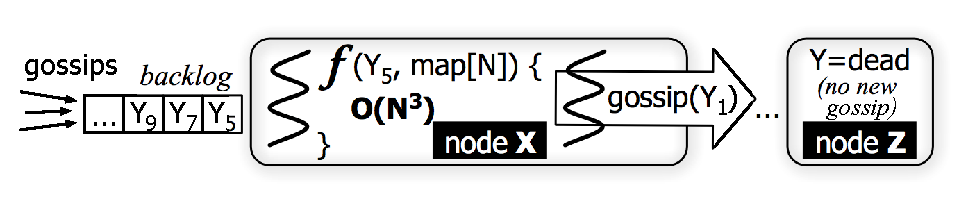
\includegraphics[height=0.8in]{F/cass1.eps}
%\includegraphics[height=0.6in]{F/empty.eps}
}
\vminfive
\mycaption[The problem of gossip-based failure detection in
Cassandra]{fig-cass1}{The problem of gossip-based failure detection in
Cassandra}{}
\vminfive
\end{figure}



We now describe in detail a control-plane scalability bug in
Cassandra, \ca{6127} \cite{CA-One}, 
% caone: jira link (see studies.tex)
which we use as a sample bug.
%
The bug surfaced on a cluster with hundreds of nodes and led to
``\textit{\textbf{flapping}}'' nodes, a condition where node up/down
status continuously changes;  tens of thousands of flaps\footnote{A 
``\textbf{flap}''
  is when a node X marks a peer node Y as down.}  were observed.




To understand this bug, we need to understand the following protocols.

\begin{enumerate}

\item {\bf Bootstrap:} Each node first creates partition keys (\eg, 32
random numbers) and gossips this information to peer nodes.
 
\item {\bf Gossip broadcast:} {\em Every second}, each node gossips to one
random node about a list of nodes and partitions it knows (including
itself) and their {\em version} numbers.  Each node also increments its
version number (``I'm still alive'') before gossiping.
 
\item {\bf Gossip processing:} The receiving node then finds any state
(metadata) differences between the two nodes to synchronize their views of
the ring.  Eventually, all nodes know about each other.
 
\item {\bf Failure detection:} {\em Every second}, a failure detection
daemon runs \cite{Lakshman+09-Cassandra}.  Put simply, if a node X has not
received a new gossip about Y {\em from anyone} (Y's version has not
changed after some period of time), X will declare Y dead (a flap).  When
X receives a new gossip about Y, it marks Y alive.

\end{enumerate}



% about the bug
There are two factors that induce the bug.  The
first is the {\em long latency of scale-dependent state-update gossip
  processing during bootstrapping} (``f'' in Figure \ref{fig-cass1}).  
While gossip processing is
usually fast in a stable cluster, it is expensive during bootstrapping as
the gossips carry many new state changes about the ring; the state-update
processing time is scale-dependent ($O(N^3)$); the larger the cluster ($N$), 
the larger the ring map, the longer the processing time is.
%
This long latency is caused by {\bf (1)} state-update checkpoint to on-disk
database and {\bf (2)} multi-map cloning and updates.
%
The first one is needed for fast fault tolerance; after a node crashes, it
can reboot fast as it knows the latest view of the ring.
%
The second one is preferred for simplicity; Cassandra clones its
\ts{MultiMap} ring table and applies changes one by one to alleviate 
long write locks.
%
% in order
% to prevent a long write lock on the ring table which can block other
% user-facing protocols.

% long
The second factor is the {\em single threaded} implementation of gossip
processing.  As shown in Figure \ref{fig-cass1},  this inability to process
multiple gossips/state updates concurrently 
(for the sake of preventing concurrency bugs) creates a {\em backlog} of new 
gossips.  For
example, in {\em every second}, Y tells someone it's alive with increasing
version number (\eg, Y$_7$), but the receiving nodes are still busy
processing state changes and only forward Y's old version number (\eg,
Y$_1$).  As Y's new gossip is not propagated on time,  other nodes
(\eg, Z) will mark Y as dead.  This happens to all
nodes, not just Y.





%http://docs.datastax.com/en/cql/3.1/cql/cql_intro_c.html


%
